% SPDX-License-Identifier: AGPL-3.0-only
% Two-column IEEEtran manuscript of the lunar AFS signal-security link-budget study.
% PRIVATE (kshana-pro). Compile: tectonic main.tex   (or pdflatex x2)
% Numbers reproduce the P1 baseline scenario in
% src/packs/lunar_signal_security_pack.rs (LunarSignalSecurityScenario::default),
% which composes the open kshana::linkbudget / kshana::jamming closed forms.
% Figure: figures/make_figures.py (same closed form, reproducible by hand).
%
% This manuscript is a neutral, results-first reframe of an earlier branded report
% ("The Lunar Navigation Signal Is Unauthenticated: ...") declined by arXiv
% moderation. Content and numbers are unchanged; the framing is academic.
\documentclass[conference]{IEEEtran}
\usepackage{graphicx}
\usepackage{booktabs}
\usepackage{amsmath}
\usepackage{url}
\graphicspath{{figures/}}

\begin{document}

\title{A Closed-Form Link-Budget Assessment of the\\
Spoofing and Jamming Attack Surface of the\\
LunaNet Augmented Forward Signal}

\author{\IEEEauthorblockN{Chakshu Baweja}
\IEEEauthorblockA{Ashforde O\"U \\ contact@ashforde.org}}

\maketitle

\begin{abstract}
The Augmented Forward Signal (AFS) that the emerging LunaNet architecture will
broadcast to lunar users carries, as currently specified, no signal-level
authentication. We quantify what that costs, in radiometric rather than rhetorical
terms, and make three contributions of graded strength. First, a closed-form
link budget: at a representative operating point the AFS reaches the lunar surface
at $-140.6$ dBW, roughly $15.6$ dB (a factor of $\sim$$36$) below the $-125$ dBW at
which terrestrial GPS L1 C/A arrives, and a multi-axis sweep of the reference and
geometry keeps the deficit inside a $12$--$18$ dB band; every term is a
cross-checked closed form (Validated). Second, an attack-surface sizing that follows
from the same budget: inverting the free-space link, a surface spoofer meeting a
$3$ dB capture criterion needs only $0.022$ mW at $1$ km, $8.9$ mW at $20$ km, and
$0.222$ W at $100$ km (denial at $30$ dB J/S costs a further $27$ dB, a factor
of $\sim$$500$); a surface attacker is bounded by the airless-body horizon
($2$ m mast $\to$ $5$ km, $1000$ m ridge $\to$ $61$ km line-of-sight reach), but a
single $\sim$$40$ W orbital transmitter meets the capture criterion over a large
sub-hemispheric cap, and no lunar signal-monitoring network exists. Third, a
sizing of the three natural defences rather than an assertion that they suffice:
an OSNMA/TESLA-style message-authentication layer is \emph{not} free, costing on the
order of $40\%$ of a representative $50$ bit/s AFS nav-data budget at first order;
an inertial/terrain cross-check bounds the residual capture a coherent spoofer can
still walk; and a sparse surveyed monitor set raises the difficulty of an
undetected wide-area attack. We are explicit about the honesty boundary: the
radiometry is Validated closed form, the service geometry and threat thresholds are
Modelled representative choices, and the whole-hemisphere reach is a uniform-beam
idealisation that a real antenna pattern narrows to a computed cap. The engine and
the figure pipeline are open under AGPL-3.0.
\end{abstract}

\section{Introduction}
Lunar exploration is converging on a shared communications-and-navigation
infrastructure. NASA's LunaNet framework, ESA's Moonlight initiative, and JAXA's
contributions are being aligned through the Interagency Operations Advisory Group
(IOAG) so that a user near the Moon can take position, navigation, and timing (PNT)
from an interoperable set of relay and navigation satellites, much as a terrestrial
user takes it from GNSS \cite{lunanet,moonlight,ioag}. A central element is the
Augmented Forward Signal (AFS): a GNSS-like ranging and navigation broadcast that a
lunar receiver acquires and tracks to fix its position and time.

Terrestrial GNSS is, by now, a well-understood single point of failure. The same
property that makes it useful, a free broadcast ranging signal, makes it spoofable
and jammable, and the feasibility of both is established in the open literature
\cite{humphreys,psiaki,tippenhauer}. The terrestrial community's answer has two
parts: authentication at the signal, exemplified by Galileo's Open Service
Navigation Message Authentication (OSNMA) \cite{osnma,osnmaicd}, and integrity
monitoring at the receiver. The lunar architecture is being specified now, before
its first operational users, which is the moment at which these lessons are
cheapest to apply.

This paper asks a narrow, quantitative question: \emph{how large is the
spoofing-and-jamming attack surface of the AFS as specified, and what would the
natural defences cost?} We answer it with a closed-form link budget and its
inverse, deliberately avoiding both alarmism and reassurance. The AFS is weaker at
the surface than terrestrial GNSS by a bounded, computable margin; that margin sets
the transmit power an attacker needs; the airless-body geometry sets where the
attacker can stand; and the defences that would close the gap are sizable rather
than free. We make three contributions of graded strength, and we tag every
number Validated (a cross-checked closed form) or Modelled (a representative
scenario or threshold input), so a reader can see exactly which claims rest on
physics and which on a service-design assumption.

\textbf{First, the received-power budget (Section~\ref{sec:budget}).} A free-space
link budget at a representative AFS operating point gives a surface received power
of $-140.6$ dBW, and a multi-axis sweep places the deficit against terrestrial GPS
in a $12$--$18$ dB band. \textbf{Second, the attack surface
(Section~\ref{sec:surface}).} Inverting the link gives the attacker transmit power
versus standoff, the horizon-limited reach of a surface attacker, and the
sub-hemispheric footprint of an orbital one. \textbf{Third, the sized defences
(Section~\ref{sec:defence}).} We size, rather than assert, a three-layer defence,
and we report the load-bearing correction that a message-authentication layer costs
on the order of $40\%$ of a representative nav-data budget, not a negligible
fraction.

\section{Related work}
\textbf{GNSS spoofing and jamming.} The feasibility of coordinated over-the-air
spoofing is established by Humphreys et al. \cite{humphreys} and, from the security
side, by Tippenhauer et al. \cite{tippenhauer}; Psiaki and Humphreys \cite{psiaki}
survey detection cues, and the TEXBAT/OAKBAT corpus \cite{texbat} provides recorded
attacks used to calibrate receivers. Jamming, the cruder denial threat, is standard
link-budget material \cite{kaplan}. This body of work is terrestrial; we import its
threat model and its J/S criteria and re-evaluate them against the lunar link.

\textbf{Signal authentication.} Galileo OSNMA \cite{osnma,osnmaicd} adds a TESLA
delayed-disclosure \cite{tesla} authentication layer to the navigation message,
the leading deployed answer to spoofing at the signal. Its cost, in bits of
overhead and in authentication latency, is documented in the OSNMA SIS ICD
\cite{osnmaicd}; we reproduce those field sizes as a terrestrial cross-check before
applying them to the AFS budget. Authentication is complementary to a receiver-side
error bound such as a timing protection level \cite{baweja2026tpl}; neither replaces
the other.

\textbf{Lunar PNT.} The LunaNet interoperability framework \cite{lunanet}, ESA
Moonlight \cite{moonlight}, and the IOAG lunar architecture \cite{ioag} specify the
service the AFS belongs to. The reference-signal parameters (received-power targets,
data rates) are still settling; we therefore treat the specific service geometry as
Modelled and expose every input, so the analysis moves with the specification rather
than freezing a number.

\textbf{Cross-sensor integrity.} Inertial and terrain-relative navigation
\cite{trn} provide an independent sensing modality that a radio-frequency spoofer
does not control; they are the lunar analogue of receiver autonomous integrity
monitoring and the basis of the second defence layer.

\section{The received-power budget}
\label{sec:budget}
\textbf{Link budget.} At a representative AFS operating point, a lunar navigation
satellite transmits $P_{\mathrm{sat}}=13$ dBW ($20$ W) through a $G_{\mathrm{sat}}=13$
dBi antenna (EIRP $=26$ dBW) at carrier $f=2.4$ GHz, and a surface user with a
$G_{\mathrm{user}}=3$ dBi antenna is at a slant range $R=3000$ km. The received power
is the standard free-space link,
\begin{equation}
P_{\mathrm{rx}} = \mathrm{EIRP} + G_{\mathrm{user}} - L_{\mathrm{fs}},
\qquad
L_{\mathrm{fs}} = 20\log_{10}\!\frac{4\pi R f}{c},
\label{eq:prx}
\end{equation}
giving $L_{\mathrm{fs}}=169.6$ dB and $P_{\mathrm{rx}}=-140.6$ dBW ($-110.6$ dBm).
Terrestrial GPS L1 C/A arrives at about $-125$ dBW \cite{isgps200,kaplan}, so the
lunar signal is $15.6$ dB weaker, a linear factor of $\sim$$36$
(Table~\ref{tab:budget}).

\begin{table}[t]
\centering
\caption{AFS surface link budget at the representative operating point. All rows
are Validated closed forms; the operating point itself is Modelled.}
\label{tab:budget}
\begin{tabular}{lrl}
\toprule
Quantity & Value & Provenance \\
\midrule
Carrier $f$                       & $2.4$ GHz       & Modelled \\
EIRP ($P_{\mathrm{sat}}+G_{\mathrm{sat}}$) & $26$ dBW & Modelled \\
Slant range $R$                   & $3000$ km       & Modelled \\
User antenna $G_{\mathrm{user}}$  & $3$ dBi         & Modelled \\
Free-space loss $L_{\mathrm{fs}}$ & $169.6$ dB      & Validated \\
Received power $P_{\mathrm{rx}}$  & $-140.6$ dBW    & Validated \\
GPS L1 C/A reference              & $-125$ dBW      & Imported \\
Power deficit                     & $15.6$ dB       & Validated \\
Deficit band (swept)              & $12$--$18$ dB   & Validated \\
\bottomrule
\end{tabular}
\end{table}

\textbf{The deficit is a band, not a point.} The $15.6$ dB headline depends on the
chosen reference and geometry, so we sweep them rather than report a single figure.
Varying the terrestrial reference over its documented spread ($-125$ to $-128.5$
dBW), the satellite EIRP, and the slant range, the deficit stays inside a
$12$--$18$ dB band (a linear factor $16$ to $63$); the rounded ``$32\times$''
($15$ dB) and the unrounded ``$36\times$'' ($15.6$ dB) are the same quantity read
to different precision. The band, computed as a multi-axis closed-form sweep over
the link inputs, is the honest object; we carry it, not the point, into the attack
surface.

\textbf{Why the deficit matters.} A jammer or spoofer is measured by the
jammer-to-signal ratio it can produce at the victim. Every decibel by which the
authentic signal is weaker is a decibel the attacker need not supply. The AFS
deficit is therefore not a vulnerability in itself but a multiplier on the one that
follows: the same attacker hardware is $12$--$18$ dB more effective against the
lunar link than against terrestrial GNSS.

\section{The attack surface}
\label{sec:surface}
\textbf{Attacker power versus standoff.} An attacker meeting a target J/S at the
victim needs a transmit power that follows from inverting the free-space link. The
J/S is referenced to the isotropic received power (the user antenna gain cancels
between the authentic signal and the attacker), so
\begin{equation}
P_{\mathrm{tx}}(d) = \big(P_{\mathrm{rx}}^{\mathrm{iso}} + \mathrm{(J/S)}\big)
+ 20\log_{10}\!\frac{4\pi d f}{c} - G_{\mathrm{tx}},
\label{eq:ptx}
\end{equation}
with $P_{\mathrm{rx}}^{\mathrm{iso}}=-143.6$ dBW and an attacker antenna
$G_{\mathrm{tx}}=6$ dBi. Under a $3$ dB capture criterion a surface spoofer needs
only $0.022$ mW at $1$ km, $8.9$ mW at $20$ km, and $0.222$ W at $100$ km; denial at
a $30$ dB J/S costs a further $27$ dB, a factor of $\sim$$500$ (so $111$ W at
$100$ km). Figure~\ref{fig:power} plots both curves. These are hand-radio power
levels: the capture threat is set by geometry and the link deficit, not by
attacker sophistication.

\begin{figure}[t]
\centering
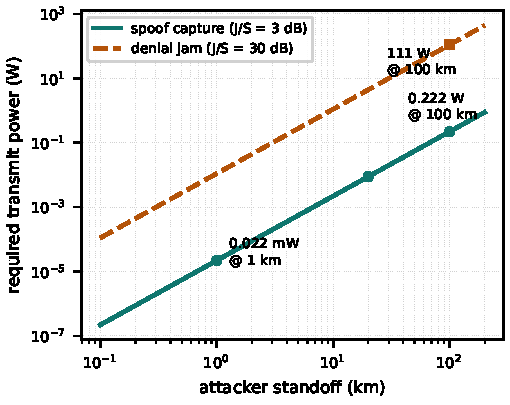
\includegraphics[width=\columnwidth]{fig1a_attacker_power.pdf}
\caption{Attacker transmit power versus standoff, from the inverse free-space link
\eqref{eq:ptx}. Spoof capture (J/S $=3$ dB, solid) and denial jamming (J/S $=30$ dB,
dashed). Markers are the reproducible anchor points ($0.022$ mW / $0.222$ W spoof at
$1$/$100$ km; $111$ W jam at $100$ km). Curves are Validated closed forms; the J/S
thresholds are Modelled.}
\label{fig:power}
\end{figure}

\textbf{The capture criterion is a modelled threshold.} We use a static $3$ dB
capture and $30$ dB denial J/S as order-of-magnitude criteria that scale the whole
table; they are Modelled inputs for an unhardened receiver, not a claimed
tracking-loop result. A pull-in model over a two-signal intermediate-frequency
stream would replace the threshold with a receiver-dynamics capture map (power
advantage $\times$ code/carrier offset $\times$ lock time); we flag this as the
principal refinement and treat the $3$ dB figure as a calibration input.

\textbf{Horizon-limited surface reach.} On an airless body a surface attacker is
bounded not by atmospheric absorption but by the geometric horizon. The
line-of-sight reach between a mast of height $h$ and a user antenna at $h_u$ is
$d = \sqrt{2R_{\mathrm{moon}}h + h^2} + \sqrt{2R_{\mathrm{moon}}h_u + h_u^2}$ with
$R_{\mathrm{moon}}=1737.4$ km; for $h_u=2$ m the reach is $5$ km from a $2$ m mast,
$8$ km from $10$ m, $21$ km from $100$ m, and $61$ km from a $1000$ m ridge
(Table~\ref{tab:horizon}). A surface spoofer is thus a local threat, its footprint
set by terrain it can climb.

\begin{table}[t]
\centering
\caption{Line-of-sight reach of a surface attacker (user antenna at $2$ m).
Validated closed-form horizon geometry on $R_{\mathrm{moon}}=1737.4$ km.}
\label{tab:horizon}
\begin{tabular}{lr}
\toprule
Attacker mast height & LOS reach \\
\midrule
$2$ m (tripod)   & $5$ km  \\
$10$ m (tower)   & $8$ km  \\
$100$ m (rim)    & $21$ km \\
$1000$ m (ridge) & $61$ km \\
\bottomrule
\end{tabular}
\end{table}

\textbf{The orbital case removes the horizon bound.} An attacker in lunar orbit is
not horizon-limited. To first order, a single $\sim$$40$ W transmitter with a $13$
dBi antenna at the AFS slant range meets the $3$ dB capture criterion across the
visible hemisphere, because it need only match the authentic EIRP plus $3$ dB and it
sees the same disk the navigation satellite does. This whole-hemisphere figure is a
uniform-beam idealisation. A real transmit antenna has an off-boresight
pattern and grazes the limb at low elevation, so the true capture region is a
sub-hemispheric cap whose edge is not captured; computing it with an Airy
aperture pattern and the limb geometry replaces ``the whole hemisphere'' with a
bounded captured fraction. Either way, the operationally important point stands: one
orbital emitter reaches a service-area-scale footprint, and there is no lunar
monitoring network positioned to see it.

\section{Sizing the defences}
\label{sec:defence}
The natural defence is layered, and the contribution of this section is to
\emph{size} each layer rather than assert that it suffices.

\textbf{Layer 1: message authentication is not free.} An OSNMA/TESLA-style layer
authenticates the navigation message by appending message-authentication codes and
disclosing keys on a delay \cite{osnma,tesla}. Reproducing the Galileo OSNMA SIS ICD
field sizes \cite{osnmaicd} as a terrestrial cross-check, the authentication content
is $120$ bit of root-key material plus $480$ bit of MAC/key per $30$ s subframe,
i.e.\ $600$ bit / $30$ s $=20$ bit/s. Against a representative AFS nav-data budget of
$50$ bit/s this is a $40\%$ first-order overhead, and the key-disclosure delay sets
a lower bound on time-to-first-authenticated-fix. We correct here an intuitive but
wrong expectation that authentication ``fits within the budget'' at a negligible
cost: at AFS-class data rates it is a first-order design load, forcing an explicit
data-rate-versus-authentication-latency trade. That the cost is sizable is itself
the finding; it does not argue against authentication, it prices it.

\textbf{Layer 2: cross-sensor integrity bounds the residual.} An inertial and
terrain-relative-navigation cross-check \cite{trn} is an independent sensing modality
a radio spoofer does not control. Composing a free-inertial coast with a
terrain fix against a spoof position/clock walk gives a minimum detectable walk rate:
the residual capture that survives authentication is bounded by how fast the spoofer
can pull the solution before the inertial/terrain monitor diverges, the lunar
instance of the timing-protection-level cross-check \cite{baweja2026tpl}. This
converts Layer 2 from an assertion into a sized bound set by the inertial and terrain
sensor noise.

\textbf{Layer 3: sparse monitors raise the wide-area cost.} A few surveyed
known-location monitor receivers, with a strong prior on expected power, timing, and
geometry, raise the probability that an orbital-scale spoof or jam is detected. The
network detection probability is $1-\prod_i(1-P_{d,i})$ over the monitors that
observe the event, a detection-theory closed form; even a sparse set materially
lowers the chance of an undetected wide-area attack, which the orbital footprint of
Section~\ref{sec:surface} otherwise makes free.

\textbf{No new physics.} None of the three layers requires a capability that does
not already exist terrestrially. The gap is one of specification and deployment: the
AFS is being defined now, and authentication, cross-sensor integrity, and monitoring
can be designed in at a fraction of the cost of retrofitting them.

\section{A per-attribute comparison, not a score}
\label{sec:compare}
Table~\ref{tab:compare} consolidates six attributes into a lunar-versus-terrestrial
comparison. We deliberately do not collapse them into a single ``security score'': a
scalar would hide which axis moved, and the axes are not commensurable. Numeric
cells derive from the Validated closed forms above; qualitative cells are Modelled
and tagged as such.

\begin{table}[t]
\centering
\caption{Six-attribute lunar-AFS-versus-terrestrial-GNSS comparison. Numeric cells
Validated; qualitative cells Modelled. No aggregate score is formed.}
\label{tab:compare}
\begin{tabular}{lll}
\toprule
Attribute & Lunar AFS & Terrestrial GNSS \\
\midrule
Received power   & $-140.6$ dBW      & $-125$ dBW \\
Signal authentication & none specified & OSNMA (Galileo) \\
Receiver cross-checks & few deployed  & RAIM, multi-const. \\
Spoof power @ 1 km & $0.022$ mW       & $\sim$$0.8$ mW \\
Monitoring network & none             & IGS, national \\
Physical access    & orbital/horizon  & widespread \\
\bottomrule
\end{tabular}
\end{table}

\section{Limitations and honesty boundary}
\label{sec:honesty}
We state the limits of the claims precisely.

\textbf{Validated means closed-form, not flight-validated.} The radiometry
(\eqref{eq:prx}, \eqref{eq:ptx}, the horizon geometry, the deficit sweep) is
Validated in the sense that each is a closed form cross-checked against the open
engine's unit tests and an independent recomputation. It is not a claim of flight
validation, certification, or agency acceptance.

\textbf{The service geometry is Modelled.} The AFS operating point (EIRP, slant
range, carrier, user antenna, nav-data rate) is a representative choice, not a frozen
specification; the LunaNet parameters are still settling. Every input is exposed so
the analysis moves with the specification. The reader should read the deficit as a
$12$--$18$ dB band and the power table as scaling with the chosen J/S criterion.

\textbf{The capture threshold is an input, not a result.} The $3$ dB capture and
$30$ dB denial J/S are order-of-magnitude criteria for an unhardened receiver. The
honest upgrade is a tracking-loop pull-in capture map; until then the power table is
threshold-scaled, and a hardened receiver moves the threshold.

\textbf{The whole-hemisphere reach is a uniform-beam idealisation.} The orbital
footprint claim assumes no antenna-pattern rolloff and no edge-of-disk grazing. A
real pattern narrows it to a computed sub-hemispheric cap; the qualitative
conclusion (one orbital emitter reaches a service-area footprint) survives, the
literal ``whole hemisphere'' does not.

\textbf{The defence sizing is first order.} The OSNMA overhead is a field-size
arithmetic against a representative data rate, not a protocol design; the Layer-2
bound depends on assumed inertial/terrain noise; the Layer-3 probability assumes
independent monitor detections. Each is a sizing to the right order of magnitude, not
an engineered defence.

\section{Conclusion}
The lunar Augmented Forward Signal, as specified, arrives at the surface $12$--$18$
dB weaker than terrestrial GPS and carries no signal-level authentication. From a
closed-form link budget we sized the consequence: a surface spoofer needs
milliwatts at kilometre standoff and is bounded only by the airless horizon, while a
single $\sim$$40$ W orbital transmitter reaches a service-area-scale footprint that
no lunar monitor is positioned to see. The natural defences are available without new
physics, but they are not free: a message-authentication layer costs on the order of
$40\%$ of a representative nav-data budget, and cross-sensor integrity and sparse
monitoring must be designed in rather than retrofitted. We reported the radiometry as
Validated closed form and the service geometry and thresholds as Modelled, and we
were explicit that the whole-hemisphere reach is a uniform-beam idealisation a real
antenna narrows. The window in which these costs are cheap to pay is the current
specification phase. The engine, the baseline scenario, and the figure pipeline are
open under AGPL-3.0 so the budget can be recomputed as the AFS specification settles.

\section*{Reproducibility}
The link budget \eqref{eq:prx}, the inverse solver \eqref{eq:ptx}, the horizon
geometry, and the deficit sweep are closed forms in the open Kshana simulator
\cite{kshana} (\texttt{kshana::linkbudget}, \texttt{kshana::jamming},
\texttt{kshana::lunar}) under AGPL-3.0, and the P1 baseline scenario reproduces
Table~\ref{tab:budget}, the power table, and Table~\ref{tab:horizon} deterministically.
The figure (\texttt{figures/make\_figures.py}) reimplements the same closed form and
prints the anchor cross-checks ($0.022$ mW @ $1$ km, $0.222$ W @ $100$ km, $111$ W jam
@ $100$ km, $-140.6$ dBW, $15.6$ dB). The OSNMA field sizes are the published Galileo
OSNMA SIS ICD values \cite{osnmaicd}, reproduced as a terrestrial cross-check.

\begin{thebibliography}{99}
\bibitem{lunanet} National Aeronautics and Space Administration, ``LunaNet
interoperability specification,'' NASA, Version 5, 2023.

\bibitem{moonlight} European Space Agency, ``Moonlight: lunar communications and
navigation services,'' ESA programme description, 2023.

\bibitem{ioag} Interagency Operations Advisory Group, ``The future lunar
communications architecture,'' IOAG Lunar Communications Architecture Study Report,
2022.

\bibitem{humphreys} T.~E. Humphreys, B.~M. Ledvina, M.~L. Psiaki, B.~W. O'Hanlon,
and P.~M. Kintner, ``Assessing the spoofing threat: development of a portable GPS
civilian spoofer,'' in \emph{Proc. ION GNSS}, 2008.

\bibitem{psiaki} M.~L. Psiaki and T.~E. Humphreys, ``GNSS spoofing and detection,''
\emph{Proc. IEEE}, vol.~104, no.~6, pp.~1258--1270, 2016.

\bibitem{tippenhauer} N.~O. Tippenhauer, C.~P\"opper, K.~B. Rasmussen, and
S.~\v{C}apkun, ``On the requirements for successful GPS spoofing attacks,'' in
\emph{Proc. ACM Conf. Computer and Communications Security (CCS)}, 2011,
pp.~75--86.

\bibitem{texbat} T.~E. Humphreys, J.~A. Bhatti, D.~P. Shepard, and K.~D. Wesson,
``The Texas spoofing test battery (TEXBAT): toward a standard for evaluating GPS
signal authentication techniques,'' in \emph{Proc. ION GNSS+}, 2012.

\bibitem{kaplan} E.~D. Kaplan and C.~J. Hegarty, \emph{Understanding GPS/GNSS:
Principles and Applications}, 3rd ed. Norwood, MA: Artech House, 2017.

\bibitem{osnma} I.~Fern\'andez-Hern\'andez, V.~Rijmen, G.~Seco-Granados, J.~Simon,
I.~Rodr\'iguez, and J.~D. Calle, ``A navigation message authentication proposal for
the Galileo open service,'' \emph{NAVIGATION}, vol.~63, no.~1, pp.~85--102, 2016.

\bibitem{osnmaicd} European Union Agency for the Space Programme, ``Galileo Open
Service Navigation Message Authentication (OSNMA) signal-in-space interface control
document (SIS ICD),'' Issue 1.1, 2023.

\bibitem{tesla} A.~Perrig, R.~Canetti, J.~D. Tygar, and D.~Song, ``The TESLA
broadcast authentication protocol,'' \emph{RSA CryptoBytes}, vol.~5, no.~2,
pp.~2--13, 2002.

\bibitem{trn} A.~E. Johnson and J.~F. Montgomery, ``Overview of terrain relative
navigation approaches for precise lunar landing,'' in \emph{Proc. IEEE Aerospace
Conf.}, 2008, pp.~1--10.

\bibitem{isgps200} Global Positioning System Directorate, ``Navstar GPS space
segment / navigation user segment interfaces,'' Interface Specification
IS-GPS-200, Rev.~N, 2022.

\bibitem{baweja2026tpl} C.~Baweja, ``A conditional timing protection level:
holdover-limited undetected time error under GNSS spoofing,'' preprint, 2026.

\bibitem{kshana} C.~Baweja, ``Kshana: an open, reproducible PNT-resilience
simulator,'' software, AGPL-3.0-only, 2026. [Online]. Available:
\url{https://github.com/ashfordeOU/kshana}
\end{thebibliography}

\end{document}
